\documentclass[conference]{IEEEtran}
\IEEEoverridecommandlockouts
\usepackage{cite}
\usepackage{amsmath,amssymb,amsfonts}
\usepackage{graphicx}
\usepackage{textcomp}
\usepackage{xcolor}
\usepackage{booktabs}
\usepackage{multirow}
\usepackage{array}
\usepackage{url}

\begin{document}

\title{AI Disaster Relief Supply Chain Optimization}

\author{
\IEEEauthorblockN{Dr. D Jeya Mala}
\IEEEauthorblockA{SCOPE \\
VIT, Chennai \\
Chennai, India \\
jeyamala.d@vit.ac.in}
\and
\IEEEauthorblockN{Sanskruti Kulkarni}
\IEEEauthorblockA{SCOPE \\
VIT, Chennai \\
Chennai, India \\
kulkarni.sanskruti.2023@vitstudent.ac.in}
\and
\IEEEauthorblockN{Jyoti}
\IEEEauthorblockA{SCOPE \\
VIT, Chennai \\
Chennai, India \\
jyoti.2023@vitstudent.ac.in}
}

\maketitle

\begin{abstract}
Disaster relief supply chains require rapid and effective allocation of limited resources under changing demand and uncertain transportation conditions. This work develops a priority-aware multi-agent reinforcement learning (MARL) framework in which three warehouse agents cooperatively dispatch water, food and medicine to five affected zones with stochastic demand growth, random road failures, limited vehicles and humanitarian priority levels. Tabular Q-Learning and SARSA, Deep Q-Network (DQN), Proximal Policy Optimization (PPO), action-masked PPO and action-masked Multi-Agent PPO (MAPPO) are compared under identical environments, rewards and training budgets, together with random and priority-greedy reference policies. A first MAPPO implementation failed to learn; diagnosis showed that a gradient-norm clip shared by the actor and the unnormalized centralized critic reduced the actor's update by about <<shrink>>$\times$, and a corrected update restored learning. On 300 held-out scenarios over three seeds, MAPPO achieved the highest reward among the learned policies (<<v2s_r>>$\pm$<<v2s_r_std>>) and reduced unmet critical demand by <<v2_vs_rnd_pct>>\% relative to random dispatching. Action masking raised PPO's reward from <<ppos_r>> to <<mps_r>> and reached the convergence threshold about <<mask_speedup>>$\times$ sooner; the centralized critic matched masked PPO's final performance with about <<std_ratio>>$\times$ lower variance across seeds and faster early learning. The tabular methods performed worse than random dispatching because their discretized state could not represent demand. A simple priority-greedy heuristic remained the best policy overall (reward <<grd_r>>, <<grd_u>> units unmet), indicating that further gains depend on reward and environment design rather than on the learning algorithm alone.
\end{abstract}

\begin{IEEEkeywords}
Disaster Relief, Humanitarian Supply Chain, Reinforcement Learning, Multi-Agent Reinforcement Learning, MAPPO, DQN, Action Masking, Supply Allocation, Demand Uncertainty, Transportation Uncertainty
\end{IEEEkeywords}


\section{Introduction}
Disasters such as floods, earthquakes, storms and other large-scale emergencies can severely disrupt transportation networks, supply facilities and access to essential resources. In such situations, humanitarian logistics plays a critical role in delivering food, water, medicine and other relief materials to affected populations. Unlike conventional supply chains, disaster-relief operations are carried out under rapidly changing conditions, limited resources, uncertain demand, damaged infrastructure and strict time constraints. Decisions about the allocation and transportation of relief supplies must therefore consider not only operational cost but also response effectiveness, equity, priority and the ability to satisfy critical requirements in a timely manner.

Emergency supply allocation is particularly challenging because the requirements of affected regions change throughout the response period. Previous studies have formulated humanitarian relief as multi-objective optimization problems involving distribution efficiency, equity, transportation capacity and the prioritization of critical victims~\cite{b1,b5}. Other approaches have incorporated realistic supply-chain considerations such as pre-positioning, procurement, backup suppliers, transportation modes and collaboration between governmental and non-governmental organizations~\cite{b4}. Although these mathematical models provide structured solutions, disaster environments can change after decisions have been made, requiring allocation policies that respond continuously to new information.

Reinforcement learning (RL) provides an alternative decision-making framework in which an agent learns suitable actions through interaction with an environment and feedback in the form of rewards. Multi-armed bandit methods have been applied to dynamic relief-supply location and allocation under disaster uncertainty~\cite{b3}, and deep RL combined with graph neural networks and digital twins has been investigated for stochastic humanitarian logistics networks~\cite{b2}. Wang et al. developed a robust deep RL framework for emergency supplies allocation under demand uncertainty using Proximal Policy Optimization (PPO)~\cite{b1}. That work considers a single response-center decision structure; extending it to several response centers introduces a coordination problem, because independent decision-makers may compete for the same demand locations or allocate resources inefficiently. Disaster conditions can also block roads, so an allocation strategy that considers demand uncertainty alone may not be sufficient.

This work studies a priority-aware MARL framework in which multiple warehouses act as cooperating agents under demand and transportation uncertainty. The contributions of this final review are:
\begin{itemize}
\item a cooperative multi-warehouse relief simulator with stochastic demand growth, random road failures, finite vehicles, three commodities and three humanitarian priority levels;
\item an implementation and comparison of Q-Learning, SARSA, DQN, PPO, action-masked PPO and MAPPO under the same environment, reward, training budget and held-out evaluation, as proposed in the initial review;
\item a diagnosis of a training failure in the initial MAPPO implementation and a corrected update rule, evaluated under an unchanged environment and reward; and
\item an analysis of the separate contributions of action masking and the centralized critic, and of the gap to a priority-greedy heuristic.
\end{itemize}


\section{Literature Survey}
Several reinforcement learning and optimization-based approaches have been explored for humanitarian logistics and disaster-relief supply allocation. The selected studies address different aspects of the problem, including demand uncertainty, dynamic allocation, transportation and network constraints, multi-objective relief distribution and simulation-based decision-making. Table~\ref{tab:lit} summarizes the relevant studies and identifies the aspects that motivate the proposed work.

\begin{table}[htbp]
\caption{Literature Survey of Disaster Relief Supply Chain Optimization Approaches}
\label{tab:lit}
\centering
\footnotesize
\renewcommand{\arraystretch}{1.15}
\begin{tabular}{|p{0.55cm}|p{1.85cm}|p{2.1cm}|p{2.1cm}|}
\hline
\textbf{Ref.} & \textbf{Method / Problem} & \textbf{Key Contribution} & \textbf{Gap / Relevance} \\
\hline
\cite{b1} & Robust DRL with PPO for emergency supply allocation under uncertain demand & Uses adversarial training, action representation and reward clipping to improve robustness under demand uncertainty. & Motivates extension toward multiple response centers, multi-agent decisions and transportation uncertainty. \\
\hline
\cite{b2} & DRL with GNNs and Digital Twins for stochastic humanitarian logistics & Combines DRL with GNN-based representation and a Digital Twin for dynamic humanitarian logistics networks. & Motivates simulation-based RL for complex logistics networks and adaptive decision-making. \\
\hline
\cite{b3} & Multi-Armed Bandits for dynamic relief allocation and location planning & Uses Geometric Greedy, $\epsilon$-Greedy and UCB for adaptive allocation and location decisions under uncertainty. & Focuses on bandit-based allocation rather than full sequential multi-agent RL, motivating broader RL comparison. \\
\hline
\cite{b4} & Humanitarian supply-chain planning with inventory, procurement, transportation and allocation & Considers realistic humanitarian supply-chain constraints and multiple planning decisions. & Primarily optimization-oriented, motivating an RL environment incorporating realistic inventory and transportation constraints. \\
\hline
\cite{b5} & Fuzzy multi-objective programming for humanitarian relief distribution & Considers priority, effectiveness, efficiency, equity, road conditions, transportation capacity and distribution constraints. & Uses mathematical optimization rather than adaptive RL, motivating priority and transportation factors in the proposed RL environment. \\
\hline
\end{tabular}
\end{table}

The reviewed studies show that both optimization and reinforcement learning can address important components of disaster-relief logistics. Existing RL-based approaches have considered demand uncertainty, dynamic allocation and complex humanitarian logistics networks, while optimization-based studies have incorporated priority, equity, transportation, inventory and other operational constraints. These aspects are generally addressed separately, which motivates a common simulation environment that combines multiple response centers, coordinated multi-agent decision-making, demand uncertainty, transportation uncertainty and priority-aware allocation.

\section{Summary of Findings and Motivation}
Existing research has demonstrated robust DRL and PPO for uncertain emergency-supply demand~\cite{b1}, DRL with graph neural networks and digital twins for complex humanitarian logistics networks~\cite{b2}, and multi-armed bandit methods for dynamic relief allocation under disaster uncertainty~\cite{b3}. Optimization-based approaches have further considered realistic supply-chain decisions and operational constraints~\cite{b4}, while multi-objective formulations have incorporated priority, efficiency, effectiveness and equity in relief distribution~\cite{b5}. The reviewed studies address these aspects through different problem formulations, leaving an opportunity to combine them within a single RL environment. This work therefore focuses on multiple response centers represented by cooperating RL agents that simultaneously face changing demand, road disruptions, limited inventories and vehicles, and priority-aware allocation, and asks whether action-constrained, coordinated MARL can learn effective allocation decisions in this setting.

\section{Proposed Methodology}
The methodology consists of a simulated disaster-relief environment, RL agents, constrained action selection, supply allocation and transportation, environment updates and performance evaluation. The overall architecture and operational flow are shown in Fig.~\ref{fig:arch} and Fig.~\ref{fig:flow}.

\begin{figure}[htbp]
\centering
\includegraphics[width=\columnwidth]{architecture.png}
\caption{Overall system architecture of the proposed multi-agent RL framework for disaster relief supply allocation.}
\label{fig:arch}
\end{figure}

\begin{figure}[htbp]
\centering
\includegraphics[width=0.78\columnwidth]{flowchart.png}
\caption{Flow diagram of the proposed RL-based disaster relief supply allocation system.}
\label{fig:flow}
\end{figure}

\subsection{Disaster Relief Environment}
The simulator contains $W=3$ warehouses, $Z=5$ affected zones and $C=3$ commodities (water, food, medicine). Each warehouse starts an episode with inventory $(500, 400, 200)$ units and four vehicles; a vehicle is consumed by each dispatch and is not returned within the episode. Each zone is assigned a humanitarian priority $p_z\in\{1,2,3\}$ (1 = critical) with probabilities $(0.25, 0.35, 0.40)$, and an initial demand $D_{z,c}$ drawn as $(140, 105, 45)\cdot\mathcal{U}(0.8, 1.2)$. Demand is non-stationary: after every step each $D_{z,c}$ grows by a Poisson increment with means $(2.0, 1.5, 0.7)$. The road network is a binary warehouse--zone availability matrix; one randomly chosen road is blocked at reset, and every open road fails permanently with probability $0.03$ per step. An episode ends after $T=20$ steps or when all vehicles are used.

\subsection{State and Action Representation}
Each agent $w$ receives a 30-dimensional local observation $o_w$: its own normalized inventory (3) and vehicle count (1), the unmet-demand ratio of every zone and commodity (15), zone priorities (5), the status of its own roads (5) and normalized time (1). The centralized critic receives a 78-dimensional global state containing all inventories, vehicles, demand, received and unmet quantities, priorities and the full road matrix.

An action selects a commodity, a destination zone and a quantity $q\in\{30, 60\}$, or a no-op, giving $3\times5\times2+1=31$ discrete actions per agent. Within a step, dispatches are executed sequentially, so a later warehouse observes the effect of an earlier one on the same zone. Only demand that is actually unmet counts as delivered; any surplus is lost.

\subsection{Action Masking}
\label{sec:mask}
Infeasible actions are removed before sampling by setting their logits to a large negative value~\cite{b9}. An action is masked when the warehouse has no vehicles left, holds no stock of the commodity, has no open road to the zone, or the zone's demand for that commodity is already satisfied. The no-op is always available.

\subsection{Priority-Aware Reward}
The shared team reward at step $t$ is
\begin{equation}
r_t = 0.05\sum_{z} \omega_{p_z}\, s_{z,t} \;-\; 0.015\, E_t \;-\; 0.08\, U^{\mathrm{crit}}_t ,
\label{eq:reward}
\end{equation}
where $s_{z,t}$ is the quantity delivered to zone $z$, $\omega_{1}=4$, $\omega_{2}=2$, $\omega_{3}=1$ are priority weights, $E_t=\sum q\,(1+0.25\,(z+1))$ is an energy/transport-cost proxy summed over dispatches (farther zones cost more), and $U^{\mathrm{crit}}_t=\sum_{z:p_z=1}\sum_c \max(D_{z,c}-R_{z,c},0)$ is the unmet demand of critical zones, with $R_{z,c}$ the quantity received. The reward was held fixed for every experiment in this report so that the comparison of training procedures is controlled.

\subsection{MAPPO Agent}
MAPPO~\cite{b6} applies PPO~\cite{b7} to cooperative multi-agent problems under centralized training and decentralized execution. All three warehouses share one actor $\pi_\theta(a\mid o_w)$, a multilayer perceptron with two hidden layers of 128 tanh units, so each agent acts only on its local observation at execution time. A centralized critic $V_\phi(s)$ of the same architecture estimates the team value from the global state during training. Advantages are computed with generalized advantage estimation (GAE)~\cite{b8} using $\gamma=0.99$ and $\lambda=0.95$ and shared across agents at each time step. The actor minimizes the clipped surrogate loss with clip ratio $0.2$ and entropy coefficient $0.01$, using 8 optimization epochs per update.


\subsection{Compared Algorithms}
\label{sec:algos}
To isolate the effect of the learning algorithm, every method controls the three warehouses with one shared learner that acts on each warehouse's local view and receives the shared team reward (independent learners with parameter sharing); only MAPPO adds a centralized critic. Following the initial review, the value-based baselines and plain PPO act without action masking: an infeasible action is executed by the environment as a no-op that consumes no vehicle.
\begin{itemize}
\item \emph{Q-Learning and SARSA}~\cite{b11}: tabular, learning rate $0.1$, $\gamma=0.99$, $\epsilon$-greedy exploration with $\epsilon$ decayed linearly from $1.0$ to $0.05$ over the first 60\% of episodes. Because the observation is continuous, the state is discretized as (own vehicles remaining, priority of each zone, status of own roads), giving at most $5\cdot3^{5}\cdot2^{5}=38{,}880$ states. Unmet demand is excluded, since even a coarse discretization of the 15 demand ratios makes the table far too large to visit.
\item \emph{DQN}~\cite{b10}: the same $2\times128$ network maps the local observation to 31 Q-values; replay buffer of 50{,}000 transitions, batch size 64, Adam ($5\times10^{-4}$), Huber loss, target network updated every 500 steps, rewards scaled by $0.1$ and the same $\epsilon$ schedule.
\item \emph{PPO}: independent PPO with a local critic $V(o_w)$ and per-agent GAE, without masking.
\item \emph{Action-masked PPO}: identical to PPO with the masking of Section~\ref{sec:mask}.
\item \emph{MAPPO}: action-masked PPO with the centralized critic $V(s)$.
\end{itemize}
All three PPO variants use the corrected update of Section~\ref{sec:fix}, so they differ only in masking and in the critic's input.

\section{Training Diagnosis and Corrected Update}
\subsection{Failure of the Initial Implementation}
The initial implementation optimized the actor and critic jointly with one Adam optimizer (learning rate $3\times10^{-4}$), clipped the combined gradient norm to $0.5$, performed one update per episode, and regressed the critic on raw returns. After 500 episodes its reward and unmet critical demand showed no trend, and its performance matched that of a random feasible policy (Table~\ref{tab:mappo}).

Instrumenting the first 50 updates explained the failure. Because episodic returns are of order $-10^{2}$, the critic's squared error was large (median <<closs>>), and its gradient norm (median <<gc>>) was about <<ratio>> times the actor's (median <<ga>>). Clipping the norm of the concatenated gradient to $0.5$ therefore scaled the actor's gradient down to a median of <<gpost>>, a reduction of about <<shrink>>$\times$, and the policy barely changed. In addition, each update used a single episode, which lasts only about four steps because the twelve vehicles are consumed quickly; normalizing advantages over roughly twelve agent-samples makes the update dominated by noise.

\subsection{Corrected Update}
\label{sec:fix}
Four changes were made to the learning procedure only; the environment and reward are identical:
\begin{enumerate}
\item separate Adam optimizers for the actor ($3\times10^{-4}$) and the critic ($10^{-3}$), each with its own gradient-norm clip of $0.5$;
\item value normalization: the critic regresses returns standardized by a running mean and standard deviation, and its output is de-normalized before GAE;
\item eight episodes are collected per update instead of one; and
\item the critic is trained on every collected state in each epoch, rather than on states sampled with replacement.
\end{enumerate}

\section{Experimental Setup}
Every algorithm was trained for 4000 episodes with three random seeds (7, 42, 123). All trained policies were evaluated on the same 300 held-out scenarios (seeds 900000--900299), which are disjoint from every training scenario. Value-based policies are evaluated greedily. Policy-gradient methods are evaluated both by sampling from the policy, which is the policy they are trained to optimize, and by taking the most probable action (argmax). Three reference policies use the same scenarios: \emph{do-nothing}, which always selects the no-op; \emph{random}, which samples uniformly among feasible actions; and \emph{priority-greedy}, a hand-written rule in which each warehouse in turn sends the largest feasible load to the zone and commodity that maximizes priority-weighted delivered quantity, with transport cost as a tie-breaker. Reported metrics are cumulative episode reward, unmet critical demand at episode end, total delivered quantity, energy proxy per episode, task completion rate (fraction of zone--commodity pairs fully satisfied), episode length in steps, and convergence speed, measured as the number of training episodes until the 100-episode moving-average training reward first reaches $-50$, a level between random dispatching and the best learned policies, averaged over seeds.

\section{Results and Discussion}

\begin{table*}[t]
\caption{Comparison on 300 Held-Out Scenarios (Learned Policies: Mean $\pm$ Std Across Three Training Seeds; n/r = Not Reached)}
\label{tab:results}
\centering
\renewcommand{\arraystretch}{1.12}
\setlength{\tabcolsep}{3.6pt}
\footnotesize
\begin{tabular}{llccccccccc}
\toprule
\textbf{Method} & \textbf{Mask} & \textbf{Eval.} & \textbf{Reward} $\uparrow$ & \textbf{Crit. unmet} $\downarrow$ & \textbf{Deliv.} $\uparrow$ & \textbf{Energy} & \textbf{Compl.} & \textbf{Steps} & \textbf{Ep. to $-50$} $\downarrow$ \\
\midrule
Do-nothing & -- & -- & <<noop_r>> & <<noop_u>> & <<noop_s>> & <<noop_e>> & <<noop_c>> & <<noop_l>> & -- \\
Random feasible & \checkmark & -- & <<rnd_r>> & <<rnd_u>> & <<rnd_s>> & <<rnd_e>> & <<rnd_c>> & <<rnd_l>> & -- \\
\midrule
Q-Learning & $\times$ & greedy & <<ql_r>> $\pm$ <<ql_r_std>> & <<ql_u>> $\pm$ <<ql_u_std>> & <<ql_s>> & <<ql_e>> & <<ql_c>> & <<ql_l>> & n/r \\
SARSA & $\times$ & greedy & <<sa_r>> $\pm$ <<sa_r_std>> & <<sa_u>> $\pm$ <<sa_u_std>> & <<sa_s>> & <<sa_e>> & <<sa_c>> & <<sa_l>> & n/r \\
DQN & $\times$ & greedy & <<dqn_r>> $\pm$ <<dqn_r_std>> & <<dqn_u>> $\pm$ <<dqn_u_std>> & <<dqn_s>> & <<dqn_e>> & <<dqn_c>> & <<dqn_l>> & <<dqn_cv>> \\
\midrule
\multirow{2}{*}{PPO} & \multirow{2}{*}{$\times$} & sampled & <<ppos_r>> $\pm$ <<ppos_r_std>> & <<ppos_u>> $\pm$ <<ppos_u_std>> & <<ppos_s>> & <<ppos_e>> & <<ppos_c>> & <<ppos_l>> & \multirow{2}{*}{<<ppo_cv>>} \\
 & & argmax & <<ppoa_r>> $\pm$ <<ppoa_r_std>> & <<ppoa_u>> $\pm$ <<ppoa_u_std>> & <<ppoa_s>> & <<ppoa_e>> & <<ppoa_c>> & <<ppoa_l>> & \\
\multirow{2}{*}{Masked PPO} & \multirow{2}{*}{\checkmark} & sampled & <<mps_r>> $\pm$ <<mps_r_std>> & <<mps_u>> $\pm$ <<mps_u_std>> & <<mps_s>> & <<mps_e>> & <<mps_c>> & <<mps_l>> & \multirow{2}{*}{<<mpp_cv>>} \\
 & & argmax & <<mpa_r>> $\pm$ <<mpa_r_std>> & <<mpa_u>> $\pm$ <<mpa_u_std>> & <<mpa_s>> & <<mpa_e>> & <<mpa_c>> & <<mpa_l>> & \\
\multirow{2}{*}{MAPPO} & \multirow{2}{*}{\checkmark} & sampled & <<v2s_r>> $\pm$ <<v2s_r_std>> & <<v2s_u>> $\pm$ <<v2s_u_std>> & <<v2s_s>> & <<v2s_e>> & <<v2s_c>> & <<v2s_l>> & \multirow{2}{*}{<<v2_cv>>} \\
 & & argmax & <<v2a_r>> $\pm$ <<v2a_r_std>> & <<v2a_u>> $\pm$ <<v2a_u_std>> & <<v2a_s>> & <<v2a_e>> & <<v2a_c>> & <<v2a_l>> & \\
\midrule
Priority-greedy & \checkmark & -- & <<grd_r>> & <<grd_u>> & <<grd_s>> & <<grd_e>> & <<grd_c>> & <<grd_l>> & -- \\
\bottomrule
\end{tabular}
\end{table*}

\begin{figure}[htbp]
\centering
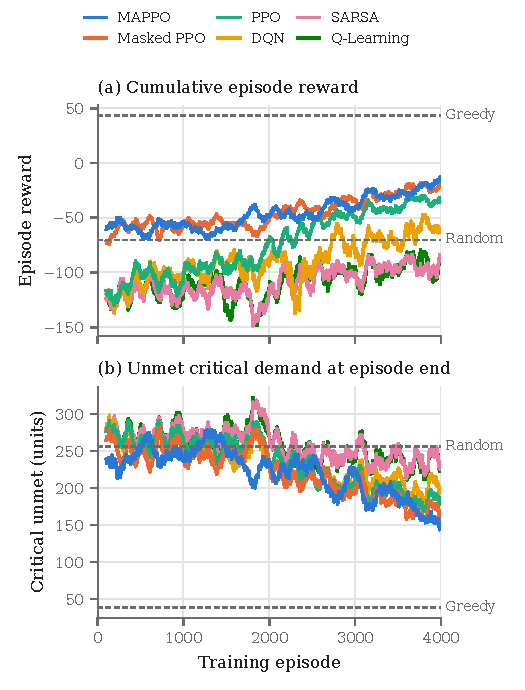
\includegraphics[width=\columnwidth]{fig_comparison.pdf}
\caption{Training curves of all algorithms (100-episode moving average, mean of three seeds). Dashed lines mark the random and priority-greedy policies evaluated on held-out scenarios. Value-based curves include $\epsilon$-greedy exploration.}
\label{fig:compare}
\end{figure}

\subsection{Overall Comparison}
Table~\ref{tab:results} and Fig.~\ref{fig:compare} compare all methods. Among the learned policies, MAPPO obtains the highest reward (<<v2s_r>>) and the lowest unmet critical demand (<<v2s_u>> units, <<v2_vs_rnd_pct>>\% below random dispatching), followed closely by action-masked PPO (<<mps_r>>, <<mps_u>> units). Ranked by reward, the order is MAPPO, masked PPO, PPO, DQN, random dispatching, Q-Learning and SARSA. The ranking compares sampled policy-gradient policies with greedy value-based policies; under deterministic (argmax) evaluation, DQN (<<dqn_r>>) and MAPPO (<<v2a_r>>) are the strongest learned policies and perform comparably given their seed-to-seed variation.

\subsection{Tabular Methods}
Q-Learning and SARSA behave almost identically and score below random dispatching in reward (<<ql_r>> and <<sa_r>> versus <<rnd_r>>), while leaving a similar amount of critical demand unmet (<<ql_u>> and <<sa_u>> units versus <<rnd_u>>). Their discretized state omits unmet demand, so the table cannot tell which zones still need supplies. The table also remains sparse: about <<ql_states>> states were visited during training, and <<ql_unseen>>\% of the states met during evaluation had never been seen (a random action is used for those). The greedy tabular policies frequently choose actions that dispatch nothing (the no-op or an infeasible action), so their episodes last <<ql_l>> steps instead of about four to five and accumulate the per-step critical-demand penalty (Section~\ref{sec:envlimits}). Their training reward never reached the convergence threshold.

\subsection{Effect of Action Masking}
Comparing PPO with action-masked PPO isolates the masking. With masking, sampled reward improves from <<ppos_r>> to <<mps_r>> and unmet critical demand falls from <<ppos_u>> to <<mps_u>> units. Masking also accelerates learning: the threshold of $-50$ is reached after <<mpp_cv>> episodes instead of <<ppo_cv>>, about <<mask_speedup>>$\times$ sooner. Without masking, each agent must discover through trial and error that blocked roads, empty inventories and satisfied demand make an action useless; masking removes those actions before sampling, as intended in the initial review.

\subsection{Effect of the Centralized Critic}
Comparing action-masked PPO with MAPPO isolates the centralized critic. Their mean final results are close (reward <<mps_r>>$\pm$<<mps_r_std>> versus <<v2s_r>>$\pm$<<v2s_r_std>>; unmet critical demand <<mps_u>>$\pm$<<mps_u_std>> versus <<v2s_u>>$\pm$<<v2s_u_std>>), and with three seeds the difference in means is within seed-to-seed variation. The centralized critic's benefits are stability and speed: the standard deviation of reward across seeds is about <<std_ratio>>$\times$ smaller, the argmax policies are far more consistent (<<v2a_r>>$\pm$<<v2a_r_std>> versus <<mpa_r>>$\pm$<<mpa_r_std>>), and the threshold is reached after <<v2_cv>> episodes instead of <<mpp_cv>>. Conditioning the value estimate on the full global state, including other warehouses' inventories and roads, is intended to reduce the variance of the advantage estimates~\cite{b6}, which is consistent with the lower seed-to-seed variance observed here.

\subsection{DQN}
DQN, evaluated greedily, reaches a reward of <<dqn_r>> and leaves <<dqn_u>> units of critical demand unmet, making it the best deterministic learner without masking. It is, however, the slowest of the neural methods to reach the threshold (<<dqn_cv>> episodes, partly because exploration decays over 60\% of training) and varies more across seeds ($\pm$<<dqn_r_std>> reward) than MAPPO.

\subsection{Diagnosis of the Original MAPPO Update}

\begin{table}[htbp]
\caption{MAPPO With the Original and Corrected Update (300 Held-Out Scenarios, Mean $\pm$ Std Across Three Seeds)}
\label{tab:mappo}
\centering
\renewcommand{\arraystretch}{1.12}
\footnotesize
\begin{tabular}{llcc}
\toprule
\textbf{Update} & \textbf{Evaluation} & \textbf{Reward} $\uparrow$ & \textbf{Critical unmet} $\downarrow$ \\
\midrule
Original & sampled & <<v1s_r>> $\pm$ <<v1s_r_std>> & <<v1s_u>> $\pm$ <<v1s_u_std>> \\
Original & argmax & <<v1a_r>> $\pm$ <<v1a_r_std>> & <<v1a_u>> $\pm$ <<v1a_u_std>> \\
Corrected & sampled & <<v2s_r>> $\pm$ <<v2s_r_std>> & <<v2s_u>> $\pm$ <<v2s_u_std>> \\
Corrected & argmax & <<v2a_r>> $\pm$ <<v2a_r_std>> & <<v2a_u>> $\pm$ <<v2a_u_std>> \\
\midrule
\multicolumn{2}{l}{Random feasible} & <<rnd_r>> & <<rnd_u>> \\
\bottomrule
\end{tabular}
\end{table}

\begin{figure}[htbp]
\centering
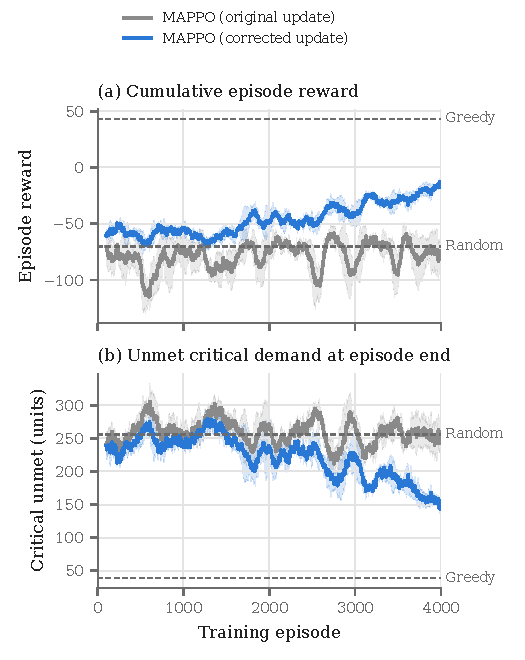
\includegraphics[width=\columnwidth]{fig_learning_curves.pdf}
\caption{Training curves (100-episode moving average; line = mean, band = $\pm$1 std across three seeds) for MAPPO with the original and corrected update. Dashed lines mark the random and priority-greedy policies evaluated on held-out scenarios.}
\label{fig:curves}
\end{figure}

Table~\ref{tab:mappo} and Fig.~\ref{fig:curves} show that, even after 4000 episodes, the original update remains at the level of random dispatching (sampled reward <<v1s_r>> versus <<rnd_r>>), and its argmax policy is worse than random. The corrected update learns steadily and reaches <<v2s_r>>. The corrected policy also delivers more relief in total (<<v2s_s>> versus <<rnd_s>> units) with the same twelve dispatches, at a higher energy cost (<<v2s_e>> versus <<rnd_e>>), consistent with sending fuller loads to zones that still have unmet demand. For all PPO variants the argmax policy is weaker than the sampled one, indicating that the learned policies still rely on stochastic action selection; sampled evaluation is therefore used for them in the main comparison.

\subsection{Comparison With the Priority-Greedy Heuristic}
The priority-greedy rule obtains a reward of <<grd_r>> and leaves only <<grd_u>> units of critical demand unmet, outperforming every learned policy by a wide margin. The rule encodes the structure of the reward directly: it always sends full loads to critical zones first. The learning agents must discover this from a noisy team signal shared across three agents, with only about four decisions per warehouse per episode. The gap shows that none of the learned policies has fully captured the priority structure, and that a strong heuristic is an essential reference point when reporting RL results for this problem.

\subsection{Environment Characteristics That Limit Performance}
\label{sec:envlimits}
Two properties of the environment bound what any policy can achieve. First, the fleet is the binding constraint: twelve dispatches of at most 60 units can deliver at most 720 units per episode, whereas mean initial demand is <<init_demand>> units and continues to grow. Task completion rate therefore stays below <<max_completion>> for every policy, including the heuristic, and is a weak metric in this configuration; unmet critical demand discriminates between policies much more clearly. Second, the critical-demand penalty in~(\ref{eq:reward}) is charged at every step, while the episode ends when the vehicles are exhausted. Dispatching quickly shortens the episode and therefore the number of penalty terms, so the reward favours speed of dispatch as well as its quality. This is visible in Table~\ref{tab:results}: the do-nothing policy, which lasts the full 20 steps, scores far below random dispatching, and the tabular policies lose most of their reward through long episodes rather than through worse allocation.

\section{Limitations and Future Work}
The progressive scenario study proposed in the initial review (fixed demand first, then demand uncertainty, transportation uncertainty and road failures) was not carried out; all results use the setting with every uncertainty enabled. Travel time is not modelled, so average response time could not be measured, and resource utilization is represented by delivered quantity. Each method was trained with three seeds, which resolves large differences but not small ones such as the mean gap between MAPPO and masked PPO. The tabular state is necessarily coarse. Future work will (i) charge the critical-demand penalty only at episode end or normalize it per step to remove the early-termination incentive, (ii) return vehicles after a travel delay so that the episode horizon and response time are meaningful, (iii) give each agent the other agents' committed dispatches or use sequential action selection to improve coordination, (iv) use the priority-greedy rule for imitation pre-training before PPO fine-tuning, and (v) run the progressive scenarios with more seeds.

\section{Conclusion}
This work developed a cooperative multi-warehouse disaster-relief simulator with stochastic demand, road failures, finite vehicles and humanitarian priorities, and compared six RL algorithms on it under identical conditions. Tabular Q-Learning and SARSA could not represent the problem and fell below random dispatching; DQN learned a reasonable deterministic policy; and the PPO family performed best. Action masking was the largest single improvement, raising PPO's reward from <<ppos_r>> to <<mps_r>> and speeding convergence about <<mask_speedup>>$\times$, while the centralized critic of MAPPO matched masked PPO's final performance with much lower variance and faster early learning. Making MAPPO train at all required correcting a shared gradient clip that let the unnormalized critic suppress the actor's update. A simple priority-greedy heuristic remains better than every learned policy, which points to reward shaping, vehicle dynamics and inter-agent coordination as the next steps toward learned policies that outperform hand-designed rules.


\begin{thebibliography}{00}
\bibitem{b1} W. Wang et al., ``When demand uncertainty occurs in emergency supplies allocation: A robust DRL approach.''
\bibitem{b2} B. Soykan and G. Rabadi, ``Optimizing humanitarian logistics with deep reinforcement learning and digital twins.''
\bibitem{b3} L. Liang et al., ``Multi-armed bandit approaches for location planning with dynamic relief supplies allocation under disaster uncertainty.''
\bibitem{b4} A. Khalili-Fard et al., ``Integrated relief pre-positioning and procurement planning for humanitarian supply chains.''
\bibitem{b5} Y. Chai et al., ``A fuzzy multi-objective programming model for the delivery and distribution of humanitarian relief materials.''
\bibitem{b6} C. Yu, A. Velu, E. Vinitsky, J. Gao, Y. Wang, A. Bayen and Y. Wu, ``The surprising effectiveness of PPO in cooperative multi-agent games,'' in \emph{Proc. NeurIPS Datasets and Benchmarks Track}, 2022.
\bibitem{b7} J. Schulman, F. Wolski, P. Dhariwal, A. Radford and O. Klimov, ``Proximal policy optimization algorithms,'' arXiv:1707.06347, 2017.
\bibitem{b8} J. Schulman, P. Moritz, S. Levine, M. Jordan and P. Abbeel, ``High-dimensional continuous control using generalized advantage estimation,'' in \emph{Proc. ICLR}, 2016.
\bibitem{b9} S. Huang and S. Onta\~{n}\'{o}n, ``A closer look at invalid action masking in policy gradient algorithms,'' in \emph{Proc. FLAIRS}, 2022.
\bibitem{b10} V. Mnih et al., ``Human-level control through deep reinforcement learning,'' \emph{Nature}, vol. 518, pp. 529--533, 2015.
\bibitem{b11} R. S. Sutton and A. G. Barto, \emph{Reinforcement Learning: An Introduction}, 2nd ed. Cambridge, MA, USA: MIT Press, 2018.
\end{thebibliography}

\end{document}
